\documentclass[a4paper, 14pt]{extarticle}

% Текст
\usepackage[utf8]{inputenc} % UTF-8 кодировка
\usepackage[russian]{babel} % Русский язык
\usepackage{indentfirst} % красная строка в первом параграфе в главе
% Отображение страниц
\usepackage{geometry} % размеры листа и отступов
\geometry{
	left=30mm,
	top=20mm,
	right=15mm,
	bottom=25mm,
	marginparsep=0mm,
	marginparwidth=0mm,
	headheight=10mm,
	headsep=7mm,
	foot=0mm}
\usepackage{afterpage,fancyhdr} % настройка колонтитулов

\setlength{\baselineskip}{1.5em}
\usepackage{titlesec}
\renewcommand{\thesection}{}
\renewcommand{\thesubsection}{\arabic{subsection}}
\titleformat{\section}[block]{\centering\bfseries\Large}{}{5pt}{}
\titleformat{\subsection}[block]{\bfseries\large}{}{5pt}{}

\pagestyle{fancy}
\fancypagestyle{style}{ % создание нового стиля style
	\fancyhf{} % очистка колонтитулов
    \fancyhead[LO, RE]{\nouppercase{DINO-Tracker}} % название документа наверху
    \fancyhead[RO, LE]{\nouppercase{\leftmark}} % название section наверху
	\fancyfoot[C]{\thepage} % номер страницы справа внизу на нечетных и слева внизу на четных
	\renewcommand{\headrulewidth}{0.25pt} % толщина линии сверху
	\renewcommand{\footrulewidth}{0pt} % толцина линии снизу
}
\fancypagestyle{plain}{ % создание нового стиля plain -- полностью пустого
	\fancyhf{}
	\renewcommand{\headrulewidth}{0pt}
}
\fancypagestyle{title}{ % создание нового стиля title -- для титульной страницы
	\fancyhf{}
	\fancyhead[C]{{\footnotesize
			
	}}
	\fancyfoot[C]{{\large 
			Санкт-Петербург, 2024
	}}
	\renewcommand{\headrulewidth}{0pt}
}

% Математика
\usepackage{amsmath, amsfonts, amssymb, amsthm} % Набор пакетов для математических текстов
\usepackage{cancel} % зачеркивание для сокращений
% Рисунки и фигуры
\usepackage{graphicx} % вставка рисунков
\usepackage{epstopdf}
\usepackage{wrapfig, subcaption} % вставка фигур, обтекая текст
\usepackage{caption} % для настройки подписей
\captionsetup{figurewithin=none,labelsep=period, font={small,it}} % настройка подписей к рисункам
% Рисование
\usepackage{tikz} % рисование
\usepackage{circuitikz}
\usepackage{pgfplots} % графики
\usepgfplotslibrary{fillbetween}
% Таблицы
\usepackage{multirow} % объединение строк
\usepackage{multicol} % объединение столбцов
% Остальное
\usepackage[unicode, pdftex]{hyperref} % гиперссылки
\usepackage{enumitem} % нормальное оформление списков
\usepackage{float}

\setlist{itemsep=0.15cm,topsep=0.15cm,parsep=1pt} % настройки списков
% Теоремы, леммы, определения...
\theoremstyle{definition}
\newtheorem{Def}{Определение}
\newtheorem*{Axiom}{Аксиома}
\theoremstyle{plain}
\newtheorem{Th}{Теорема}
\newtheorem{Task}{Задание}
\newtheorem{Lem}{Лемма}
\newtheorem{Cor}{Следствие}
\newtheorem{Ex}{Пример}
\theoremstyle{remark}
\newtheorem*{Note}{Замечание}
\newtheorem*{Solution}{Решение}
\newtheorem*{Proof}{Доказательство}
% Свои команды
\newcommand{\comb}[1]{\left[\hspace{-4pt}\begin{array}{l}#1\end{array}\right.\hspace{-5pt} } % совокупность уравнений
\newcommand{\rank}{\mathrm{rank}\;}
% Титульный лист

\usepackage{listings}
\newcommand*{\titlePage}{
	\thispagestyle{title}
	\begingroup
	\begin{center}
		%		{\footnotesize
			%			Министерство образования и науки Российской Федерации\\
			%			Федеральное государственное автономное образовательное учреждение высшего образования
			%		}
		%		
		\vspace*{3ex}
		{\small
		}
		
		\vspace*{2ex}
		
		{\normalsize
		}
		
		\vspace*{30ex}
		
		{\Large \bfseries 
			Отчёт о выполнении тестового задания\\
			{\large <<DINO-Tracker: Taming DINO for Self-Supervised
			Point Tracking in a Single Video>>\\
				}
			
		}
		
	\end{center}
	\vspace*{10ex}
	\begin{flushright}
		{\large 
			\underline{Выполнил}: \textbf{Дюжев В. Д.}
		}

	\end{flushright}	
	\newpage
	\setcounter{page}{1}
	\endgroup}
%\usepackage{newtxmath,newtxtext}
%\lstset{literate={а}{\cyra}1{б}{\cyrb}1{в}{\cyrv}1{г}{\cyrg}1{д}{\cyrd}1{е}{\cyre}1{ж}{\cyrzh}1{з}{\cyrz}1{и}{\cyri}1{к}{\cyrk}1{л}{\cyrl}1{м}{\cyrm}1{н}{\cyrn}1{о}{\cyro}1{п}{\cyrp}1{р}{\cyrr}1{с}{\cyrs}1{т}{\cyrt}1{у}{\cyru}1{ф}{\cyrf}1{х}{h}1{ц}{w}1{ч}{\cyrch}1{ш}{\cyrsh}1{щ}{\cyrshch}1{ь}{m}1{ъ}{m}1{ы}{y}1{э}{e}1{ю}{\cyryu}1{я}{\cyrya}}

\lstset{basicstyle=\small}
\newcommand{\tasknum}[3]{Task}%\textunderscore{#1}\textunderscore{#2}y\textunderscore{#2}\textunderscore{#3}}
\usepackage{pdfpages}

\newcommand{\mat}[1]{\begin{pmatrix}#1\end{pmatrix}} 
\newcommand{\bmat}[1]{\begin{bmatrix}#1\end{bmatrix}} 

\newcommand{\code}[2]
{
\begin{minipage}{0.45\textwidth}
    \textbf{Code:}
    #1
\end{minipage}
}

\begin{document}
\renewcommand{\contentsname}{\hfillОГЛАВЛЕНИЕ\hfill} 
\titlePage
\thispagestyle{plain}
\tableofcontents
\pagestyle{style}

\newpage
\setcounter{page}{1}


\section{Введение}
\subsection{Краткое описание}
Dino-Tracker --- метод трекинга, созданный на основе DINOv2-ViT, которая используется как базовая модель для получения качественных векторов-обобщений для изображений, содержащих важную семантическую информацию. Он позволяет добиться высокой точности, при этом относится к области self-supervised learning, что расширяет возможности его использования (т.к. нет необходимости разметки данных). Перед применением предполагается обучение на конкретном видео.

\subsection{Постановка задачи}
Дана последовательность кадров $\{I^t\}^T_{t=1}$, где $T$ --- длина видео. Задача состоит в обучении модели-трекера $\Pi$, принимающего на вход целевую точку $x_q$ (query point) и предсказывающего набор $\{\hat{x}^t\}^T_{t=1}$ --- траекторию данной точки (положения на всех кадрах). Целевая точка при этом задается положением и кадром (далее --- начальный кадр).
Таким образом итоговым результатом является возможность предсказания траектории любой точки любого кадра на протяжении всего видео.

\subsection{Структура отчета}
Данный отчет состоит из 5 секций:
\begin{enumerate}
	\item \textbf{Запуск предобученной модели} --- содержит базовые результаты экспериментов с демонстрацией основных возможностей метода на предложенных в оригинальном репозитории данных.
	\item \textbf{Принцип работы} --- описание арихитектуры нейросетевой модели и алгоритмов постобработки, а также процесса обучения.
	\item \textbf{Запуск на собственных данных} --- результаты обучения модели на собранных вручную реальных данных.
	\item \textbf{Техническая информация} --- описание процесса взаимодействия с ПО, дополнения к оригинальному репозиторию.
	\item \textbf{Выводы} --- подведение итогов, выдвижение гипотез для улучшения метода.
\end{enumerate}

\newpage

\section{Запуск предобученной модели}
В данной секции представлены результаты использования модели DINO-Tracker на последовательностях из датасета 
Tapvid-Davis-480. Данные доступны по \href{https://www.dropbox.com/scl/fo/7s2rgsm92qbzzh2xnx51d/AIvXxRaJPL2RQm43Zi_taJU?e=1&preview=davis_480.zip&rlkey=6cs0bm2u0on1u7z0jyxlq8avq&st=7s75r77a&dl=0}{ссылке}, указанной в репозитории.
\subsection{Базовая визуализация}
В качестве примеров для демострации работоспособности базовой модели DINO-Tracker (предсказаний нейросетевой части, без постобработки) были выбраны видео-последовательности с достаточно простым профилем движения, без явных окклюзий. На рисунках \ref{fig:davis-29}-\ref{fig:davis-21} изображены по 3 кадра (первый, центральный и последний) с демонстрацией промежуточных траекторий для целевых точек (начальным кадром во всех случаях является первый).
\begin{figure}
    [H]
    \centering
    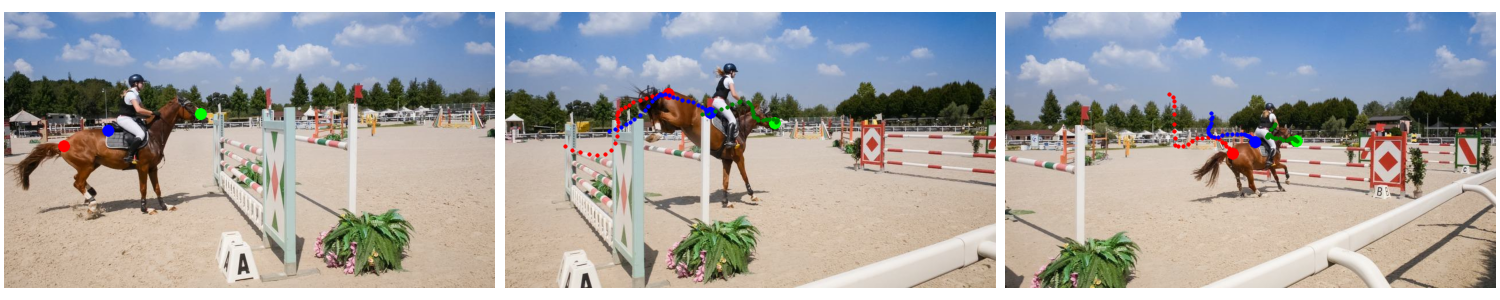
\includegraphics[width=\textwidth]{figs/davis-29.png}
    \caption{Траектории DINO-Tracker. Tapvid-Davis-480/29.}
    \label{fig:davis-29}
\end{figure}
\begin{figure}
    [H]
    \centering
    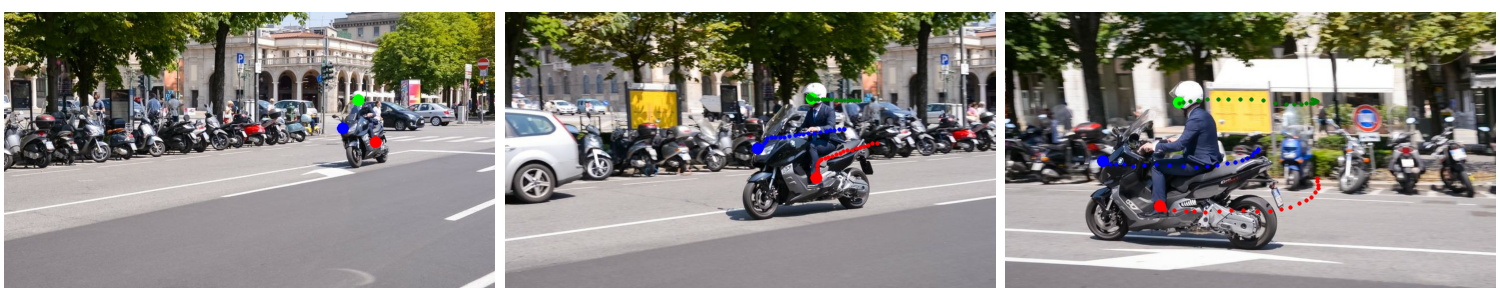
\includegraphics[width=\textwidth]{figs/davis-26.png}
    \caption{Траектории DINO-Tracker. Tapvid-Davis-480/26.}
    \label{fig:davis-26}
\end{figure}
\begin{figure}
    [H]
    \centering
    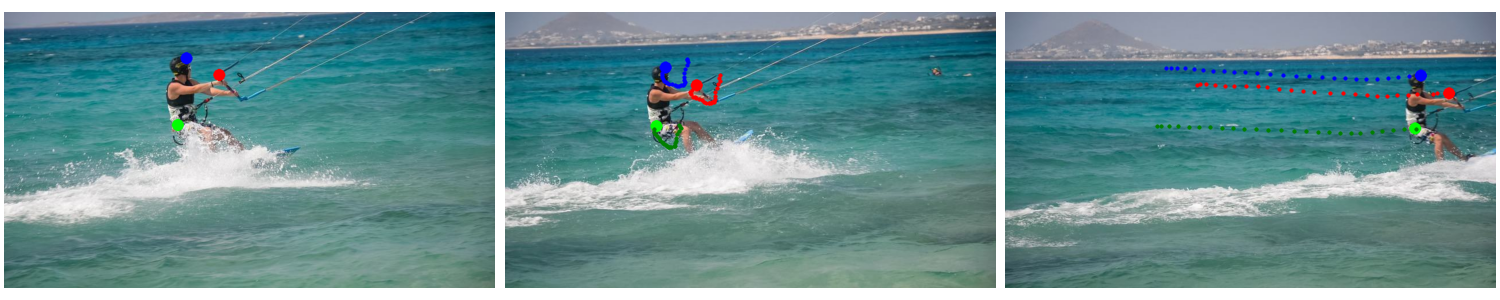
\includegraphics[width=\textwidth]{figs/davis-21.png}
    \caption{Траектории DINO-Tracker. Tapvid-Davis-480/21.}
    \label{fig:davis-21}
\end{figure}

Можем заметить, что полученные траектории имеют естественный вид. 
Базовый метод может быть успешно применен и к трекингу в более сложных окружениях 
(рисунок \ref{fig:davis-13}), однако важно чтобы целевая точка находилась в достаточно 
уникальной части изображения и не подвергалась окклюзиям. Например, на рисунке 
\ref{fig:davis-15} видно, что целевая точка сопоставляется неправильно с определенного 
момента времени (из-за появления схожего объекта и окклюзии вервоначальной цели). 
Данные ограничения помогает во многом снять постобработка с предсказанием окклюзий, 
о которой будет сказано в дальнейшем.

\begin{figure}
    [H]
    \centering
    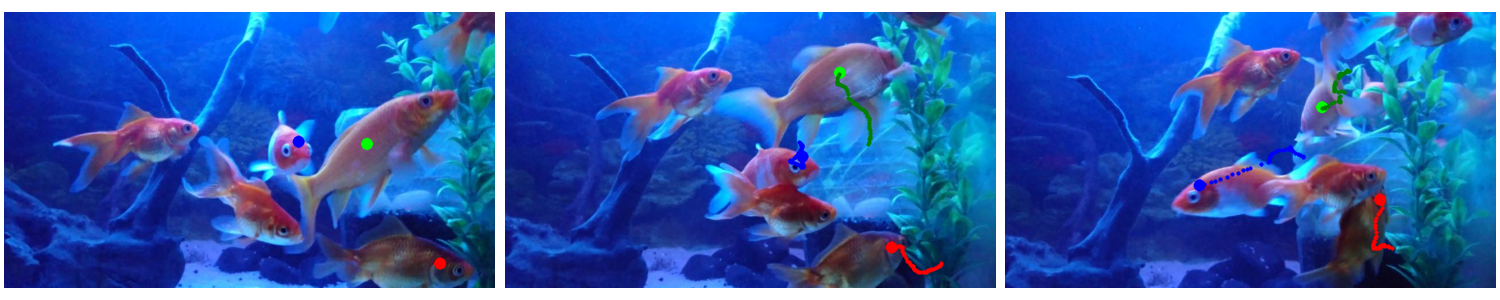
\includegraphics[width=\textwidth]{figs/davis-13.png}
    \caption{Траектории DINO-Tracker. Tapvid-Davis-480/13.}
    \label{fig:davis-13}
\end{figure}
\begin{figure}
    [H]
    \centering
    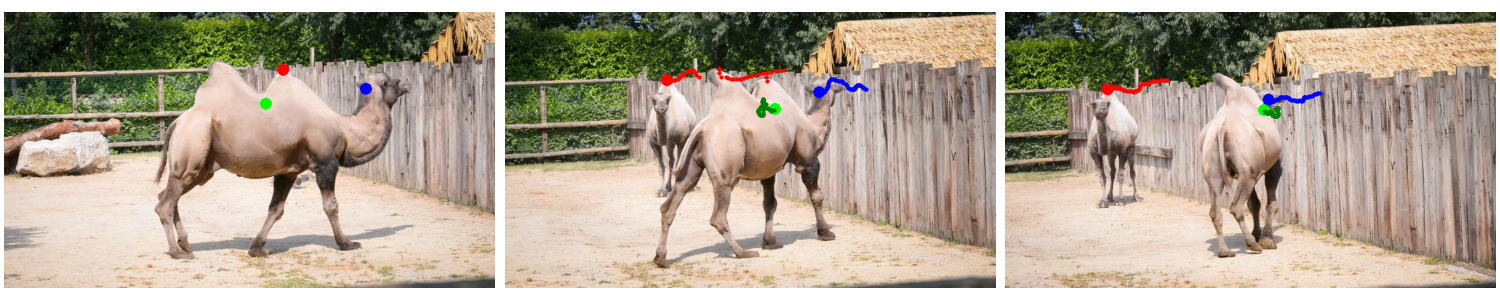
\includegraphics[width=\textwidth]{figs/davis-15.png}
    \caption{Траектории DINO-Tracker. Tapvid-Davis-480/15.}
    \label{fig:davis-15}
\end{figure}

\subsection{Метрики качества}

Оценка качества трекинга производится на датасете Tapvid-Davis-480 согласно инструкции, указанной в репозитории (также есть возможность провести оценку на других предложенных наборах данных, однако ввиду длительности процесса был выбран один из них).

Для оценки исполбзуются метрики, предложенные в оригинальной статье <<TAP-Vid: A Benchmark for Tracking Any Point in a Video>>: 
\begin{enumerate}
    \item occlusion accuracy ($OA$) --- отношение количества правильно предсказанных окклюзий в последовательности к длине последовательности (стандартная accuracy классификации);
    \item position accuracy ($<\delta^x$) --- отношение количества правильно предсказанных положений видимых точек (без окклюзий) последовательности к количеству видимых точек, где правильными считаются предсказания, лежащие в заданной окрестности (в пикселях) действительных значений;
    \item jaccard --- объединенная метрика для оценки качества предсказаний окклюзий и положений, рассчитываемая как отношение количества правильно предсказанных положений видимых точек с соответствующим правильным предсказанием окклюзий последовательности к количеству видимых точек + количеству неправильно классифицированных невидимых точек или точек с неправильными предсказаниями положений, предсказанных видимыми.
\end{enumerate}
Важно отметить, что метрики $<\delta^x$ и jaccard рассчитываются для всех изображений последовательности (кроме начальных для соответствующих ключевых точек) с учетом приведения к размеру 256x256.
В качестве итоговых метрик выступают $OA$, average jaccard ($AJ$) и average position accuracy ($<\delta^x_{avg}$), где поледние две расчитываются как средние значения jaccard и $<\delta^x$ для окрестностей в 1, 2, 4, 8 и 16 пикселей.
\begin{table}[!ht]
    \centering
    \begin{tabular}{|l|l|l|l || l|l|l|l|}
    \hline
	\textbf{id} & \textbf{$OA$} & \textbf{$AJ$} & \textbf{$<\delta^x_{avg}$} & \textbf{id} & \textbf{$OA$} & \textbf{$AJ$} & \textbf{$<\delta^x_{avg}$} \\ \hline
        25 & 0.86407 & 0.52461 & 0.71564 & 23 & 0.88914 & 0.70477 & 0.8492 \\ \hline
        7 & 0.84293 & 0.62454 & 0.82839 & 14 & 0.95139 & 0.64647 & 0.75761 \\ \hline
        20 & 0.83599 & 0.5811 & 0.77156 & 13 & 0.89146 & 0.59985 & 0.72462 \\ \hline
        1 & 0.83536 & 0.55336 & 0.77867 & 29 & 0.96237 & 0.78638 & 0.87435 \\ \hline
        26 & 0.92519 & 0.72271 & 0.84825 & 17 & 0.89871 & 0.61162 & 0.75912 \\ \hline
        5 & 0.87887 & 0.60303 & 0.8446 & 4 & 0.87391 & 0.66864 & 0.88173 \\ \hline
        2 & 0.69653 & 0.37687 & 0.72344 & 11 & 0.79149 & 0.57035 & 0.7935 \\ \hline
        19 & 0.82501 & 0.47515 & 0.70126 & 16 & 1.0 & 0.94087 & 0.96645 \\ \hline
        6 & 0.85056 & 0.63005 & 0.80656 & 10 & 0.94926 & 0.76182 & 0.86853 \\ \hline
        22 & 0.79057 & 0.54181 & 0.76219 & 3 & 0.91635 & 0.75579 & 0.8585 \\ \hline
        8 & 0.88787 & 0.69386 & 0.84002 & 21 & 0.98371 & 0.84777 & 0.90917 \\ \hline
        28 & 0.93551 & 0.73576 & 0.84587 & 24 & 0.94805 & 0.8512 & 0.9379 \\ \hline
        0 & 0.99963 & 0.64083 & 0.72042 & 15 & 0.96577 & 0.80356 & 0.87399 \\ \hline
        9 & 0.69041 & 0.29614 & 0.5251 & 18 & 0.81178 & 0.52368 & 0.71774 \\ \hline
        27 & 0.87957 & 0.62347 & 0.7801 & 12 & 0.99365 & 0.88775 & 0.93579  \\ \hline
        \hline
        \textit{\textbf{avg}} & \textit{\textbf{0.8855} }& \textit{\textbf{0.65279}} & \textit{\textbf{0.80668}} & --- & --- & --- & --- \\ \hline
    \end{tabular}
	\caption{Метрики качества. Датасет Tapvid-Davis-480.}
\end{table}

В статье завлены следующие данные для рассматриваемого датасета:
$OA=0.881, AJ=0.646, <\delta^x_{avg}=0.804$. Эксперимент подтверждает достижение таких значений.
	
\subsection{Производительность}
Эксперименты производятся на устройстве Lenovo Legion 7 (AMD Ryzen 9 5900HX, NVIDIA GeForce RTX 3080 120W 16Gb, 32 Gb RAM).

Для получения данных о производительности в инференсе метод был применен ко всем последовательностям из датасета. Эксперимент проводился только для нейросетевой части DINO-Tracker. Дальнейшее предсказание окклюзий сильно зависит от контекста изображения.
На вход модели подавалась одна ключевая точка, соответсвующая центру первого кадра. Принятый размер батча: $1$.
Ниже приведен график, иллюстрирующий зависимость времени обработки видео от количества кадров в нем. 
\begin{figure}
    [H]
    \centering
    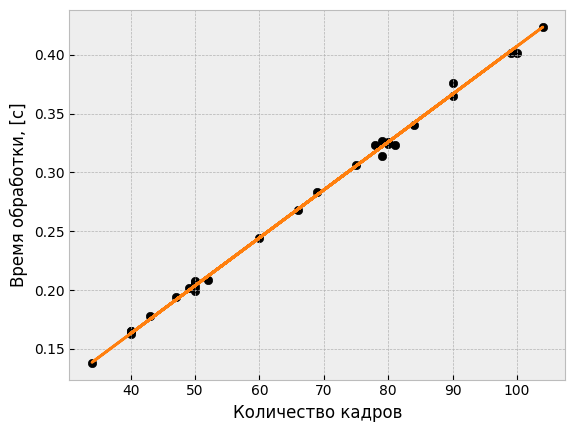
\includegraphics[width=\textwidth]{figs/performance.png}
    \caption{Зависимость времени инференса нейросетевой части DINO-Tracker от количества кадров.}
    \label{fig:performance}
\end{figure}

Алгоритм обработки видео последовательно предсказывает положение целевой точки на кадрах. Данные подтверждают, что зависимость является линейной. Аппроксимировав ее моделью линейной регрессиии без смещения получим, что на предсказание позиции целевой точки в одном кадре тратится в среднем $0.0041$ [с].

В процессе инференса в среднем затрачивалось 14.5 Гб видеопамяти.

\subsection{Мульти-трекинг}

\end{document}
\input{metrics_table}

